\chapter{Spatial-Spark计算框架}{Spatial-Spark Computation Framework}
\section{空间数据分析处理}{Procession of Spatial Data}
\subsection{空间数据格式}
空间数据量大且空间数据格式也是各式各样。开放地理空间信息联盟(Open GIS 
Consortium, OGC)定义了一些空间矢量数据格式\cite{Bychowski2003Open},方便能够进行空间数据分析
处理和交换,下面介绍几种常用的空间矢量数据格式。

(1)WKT数据格式

WKT(Well-Know-Text)数据格式以文本形式描述,用来表示点,线和面空间对象,见表\ref{tab:wktdata}。
\begin{table}
    \centering
    \caption{WKT矢量空间数据}{Vector spatial data in WKT}
    \label{tab:wktdata}
    \tabulinesep=1.5mm
    \begin{tabu}to 0.8\linewidth{X[1.1,c]X[2.5,c]}
        \tabucline[0.10em]-
        \rowfont[c]{} 几何类型 & WKT表示方式 \\
        \tabucline-
        ST\_Point & POINT(10.05 10.28) \\
        ST\_LineString & LINESTRING (10.05 10.28 , 20.95 20.89) \\
        ST\_Polygon & POLYGON((10 10, 10 20, 20 20, 20 15, 10 10)) \\
        \tabucline[0.10em]-
    \end{tabu}
\end{table}

(2)GeoJSON数据格式

GeoJSON数据是通过JSON数据表达简单的数据格式,如点、线、多边形和这些几何类型的集合以及他们非空间属性信息,表达方式如下:
\begin{lstlisting}[
  morekeywords={type,geometry,coordinate,fields}
]
{
  "type":"feature",
    "geometry":{
      "type":"LineString",
        "coordinate":[[[-100.50,57.14],[-89.45,62.17],[-37.21,79.73]]],
        "fields":{
            "prop1":"value","prop2":"string"
            }                
    }
}
\end{lstlisting}

由于JSON格式在序列化和网络传输中的优势,非常适合分布式的数据存储,空间数据和属性数据都存储在普通的文本中。

(3)GML数据格式  

GML(Geography Markup Language)是以XML格式的空间数据表达形式,并使用XML Schema文件
定义技术,目前版本为$2.1.1$。XML Schema具有类型继承、命名空间等特性,通过XLink来表现地理空间实体的关系。
\begin{lstlisting}[language=XML]
<PhotoCollection xmlns="http://www.myhotos.org"
    xmlns:gml="http://www.opengis.net/gml"
    xmlns:xsi="http://www.w3.org/2001/XMLSchema-instance"
    xsi:schemaLocation="http://www.myphotos.org" >
    <items>
      <item>
        <name>Lynn</name>
          <description>A shot of the falls</description>
          <where>North Vancouver</where>
          <position>
            <gml:Point srsDimension="2" 
              srsName="http://www.opengis.net/def/crs/EPSG/0/4326" >
                <gml:pos>49.40 -123.26</gml:pos>
            </gml:Point>
          </position>
      </item>
    </items>
</PhotoCollection>
\end{lstlisting}

\subsection{空间数据转换}
空间数据来源各异,每种数据来源有各自的坐标参考系统,如GPS接收机获取的地理空间数据
是以WGS$84$坐标系统为基准;摄影测量往往采用该区域最适宜的坐标参考系统为基准。不同的
大地坐标系统和平面投影系统往往使得空间数据处理和分析正确性得不到保证,因此很有必要
将多源空间数据纳入到同一个空间参考系统下。

Proj.$4$是开源GIS中著名的地图投影库\cite{Urbanek2012proj4},在GRASS GIS, MapServer, PostGIS等众多GIS
软件中都直接或者间接使用Proj.$4$,$2008$年OSGeo将Proj.$4$纳入到MetaCRS的一部分,Proj.$4$
的主要功能是提供了大地坐标系和投影坐标之间的正反算,不同参考基准的坐标变换。Proj.$4$使
用C语言编写,但不同的语言也有各自相应的Proj.$4$库,如Java语言的Proj$4$j,C\#语言的Proj$4$.Net,JavaScript语言
的Proj$4$js等等。

以Java语言的Proj$4$j库为例,Proj$4$j 主要模块的如下:

(1)Datum基准

定义了空间椭球基准,主要参数包括椭球的名称,长半轴和短半轴,以及质心偏离中心的位置,Proj4j
内置了若干个常用的椭球基准如WGS84,IRE65等。

(2)CoordinateReferenceSystem参考系统

不同的坐标参照系统需要指定不同的参数,如高斯投影的坐标参考系统需要指定中央经度和投影带宽度,而
兰伯特投影需要指定投影的第一纬度、第二纬度,中央纬度和中央经度。

(3)Projection投影

Proj4j提供了$96$种投影方式,Projection是这些投影类的基类,每个投影类提供了project函数和projectInverse
函数,分别代表了投影正算和投影反算。

(4)CoordinationTransform坐标换算

坐标转换提供了不同坐标参考系统之间坐标换算类,如将高斯投影坐标换算兰伯特投影坐标,通过两个坐标参考系统
对象创建坐标换算类,生成CoordinationTransform对象,调用transform函数完成坐标换算。

\subsection{空间数据分析}
空间数据分析的正确性是GIS的一个重要参照指标,尤其在涉及空间数据数据几何拓扑关系时需要严格正确。JTS Topology Suite
是加拿大Vivid Solutions公司提供的一套开源的空间几何对象拓扑操作工具包,主要包含的功能和特色如下:

(1)实现了OGC关于简单要素的SQL查询规范定义的空间数据模型。

(2)完整的、一致的和基本的二维空间算法的实现,包含了空间分析和空间运算\cite{Johansson2002Using}。

(3)提供了常见的空间数据格式读写接口。

JTS Topology Suite在GIS中最重要的应用是计算两个几何对象之间的空间拓扑关系,每个派生自Geometry类的几何
对象都能够进行相互空间分析和空间运算,详细见表格\ref{tab:spatialanalysisoperation}。
\begin{table}
  \centering
  \caption{空间分析和空间运算}{Spatial analysises and spatial operations}
  \label{tab:spatialanalysisoperation}
  \tabulinesep=1.5mm
  \begin{tabu} to 1.0 \linewidth{X[1,c,m]X[1.4,c,m]X[2,c,m]|X[1,c,m]X[1.4,c,m]X[2,c,m]}
  \tabucline[0.1em]-
  类别 & 函数 & 功能 & 类别 & 函数 & 功能 \\
  \tabucline-
  \multirow{6}{*}{空间分析} & Contain & 包含关系 & \multirow{2}{*}{空间分析} & Overlap & 重叠关系 \\
  	& Equal & 相等关系 &  &Touch & 相接关系  \\
	\tabucline{4-6}
	& Intersect & 相交关系 & \multirow{4}{*}{空间运算} & Buffer & 缓冲区运算 \\
	& Within & 内部关系 &	& Intersection & 交集运算\\
	& Disjoint & 相离关系 & 	& Difference & 差集运算 \\
	& Cross & 内部相交关系 &  & Union & 并集运算\\
\tabucline[0.10em]-
\end{tabu}
\end{table}

\section{RDD空间扩展}{Spatial Extension of RDD}
空间数据爆炸式增长对空间数据处理提出了新的挑战,主要有以下两点:\circled{1}系统可扩展性(System Scalability):
数据的存储、读取和写入能够有效地处理GB、TB级别甚至PB级数据;\circled{2}交互式高性能(Interactive Performance):
在处理空间数据查询后,能够高效回应查询请求\cite{Yu2015GeoSpark}。

\subsection{空间数据类型}
Spark采用抽象数据类型RDD,通过分布式平行数据结构处理海量数据,使用独特的内存计算使得在处理数据
方面有着较高的性能优势。但是RDD没有完善的空间数据支持和空间操作,因此开发人员需要在Spark提供API上层重新定义空
间数据读写和操作函数,但这些没有统一的标准。

为了在分析海量空间数据时能够专注于分析算法,本文设计出一套海量空间数据分析框架:Spatial-Spark。Spatial-Spark扩展
了Spark RDD,使之能够支持常见的空间数据类型、空间索引和空间操作,整个Spatial-Spark体系结构见
图\ref{fig:spatialsparkarchitecture},底层为数据存储层,核心部分为中间Spatial-RDD空间几何对象层,最上层为
空间分析层,提供了高度定制的API接口。
\begin{figure}
  \centering  
  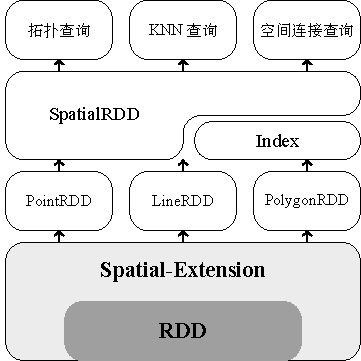
\includegraphics{figures/spatialspark.pdf}\\
  \caption{Spatial-Spark体系架构}{Spatial-Spark architecture}
  \label{fig:spatialsparkarchitecture}
\end{figure}

空间数据类型是Spatial-Spark的核心,通过RDD将点、线和面分别封装成PointRDD、LineRDD和PolygonRDD。这些Spatial-RDD表
示在集群中并行分区存储空间几何对象的集合,主要有两种方式生成Spatial-RDD:\circled{1}从HDFS中读取数据,主要流程见图\ref{fig:spatialrdd},文本空间
数据以行记录存储在HDFS中,先经过文件格式装换,将WKT,GeoJSON等数据转换成空间对象,再空间数据坐标参考系统转换统一,最
后生成Spatial-RDD,其中转换和投影步骤以接口形式提供,用户可以重写接口,完成定制化需求;\circled{2}Spatial-RDD相互之间空间运算,如PointRDD
可以通过缓冲区操作生成PolygonRDD对象,PolygonRDD对象通过提取重生成PointRDD。
\begin{figure}
\centering
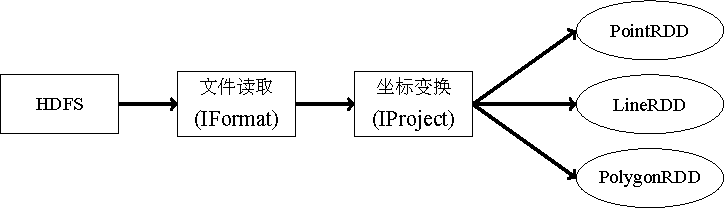
\includegraphics[scale=0.9]{figures/spatialRDD.pdf}
\caption{HDFS生成Spatial-RDD流程}{Generating Spatial RDD from HDFS} 
\label{fig:spatialrdd}
\end{figure}


\subsection{空间数据索引}
\subsubsection{RDD分区}
RDD内部数据集合在逻辑上(以及物理上)被划分为多个小集合,这样每个小集合就被成为分区。以图\ref{fig:rddpartition}为例,
RDD1有五个分区(Partition),分布在四个DataNode上面,而RDD2有三个分区,分布在
三个DataNode上面。在源码级别,RDD类存储一个Partition列表,每个Partition对象都包含
一个index成员,通过RDD编号加index就能从唯一的分区的Block编号\cite{Zaharia2012Resilient},持久化的RDD就能通过这
个Block变化从HDFS中获取对应的分区数据。
\begin{figure}
\centering
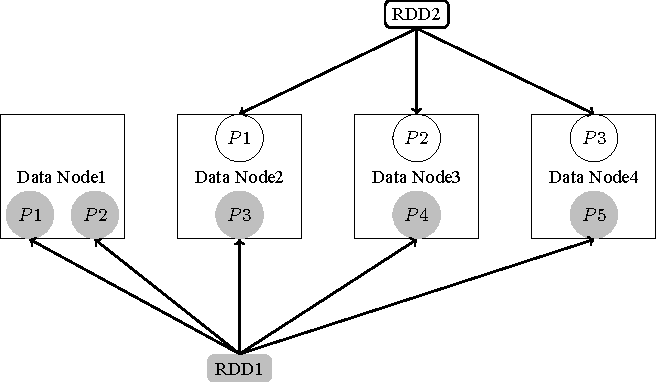
\includegraphics[scale=0.8]{figures/rddpartition.pdf}
\caption{RDD分区}{RDD partition illustration}
\label{fig:rddpartition}
\end{figure}

分区的个数决定了并行计算的粒度,多个分区能够并行计算,充分利用分布式计算资源。通常来讲,分区
的数量为计算集群的CPU核心数量的$3-4$倍。创建分区的方法主要有两种:\circled{1}在SparkContext对象读取数据
的时候指定分区的数量;\circled{2}调用RDD的分区器函数,进行重新分区。Spark在读取数据时默
认使用哈希分区器,该分区器实现简单,运算速度快,但缺点是不关心键值的分布情况,其散列到不同分区的概率会
因数据而异。往往会带来分区负载的不平衡性。

考虑到空间数据空间分布特点,Spatial-Spark提供了空间分区,重写了Partitioner函数,能够尽可能
将空间上分布相邻的空间对象处于同一RDD分区。具体算法步骤如下:

(1)根据空间要素集合的边界(boundary)和分区数量n,将整个boundary划分为$\sqrt{n}\times \sqrt{n}$个
网格,每个网格拥有一个id值。

(2)将\verb|RDD<Geometry>|进行Map或者MapPartition操作,使之转换为PairRDD<Integer,Geometry>描述
的Key-Value对象,其中Key为网格中与其相交或者包含的网格的id值,如果有多个网格与之相交,取其中一个。

(3)对\verb|PairRDD<Interger,Geometry>|按照key进行重分区计算,使每个分区能够拥有分布较为均匀的
几何对象,而且尽量保证相邻的空间的对象在同一个分区。

\subsubsection{分区索引}

好的空间索引能够极大地方便海量空间数据查询,而空间数据中最常用的空间数据索引方式就是R树。R树索引是有
美国加州大学Guttman A.教授提出的一种空间数据库的动态索引算法\cite{Guttman1984R},该数据结构的核心思想是通
过最小外包矩形(Minimum Bounding Rectangle, MBR)表达一个或者一组空间几何对象。与B树一样,R树是一棵高度平衡树,
将所有的空间几何对象都存放在叶节点,插入和删除节点不需要完全重构R树,只需要在局部进行相关拓扑调整即可,
一棵典型的R树如图\ref{fig:rtree}所示。
\begin{figure}
\centering
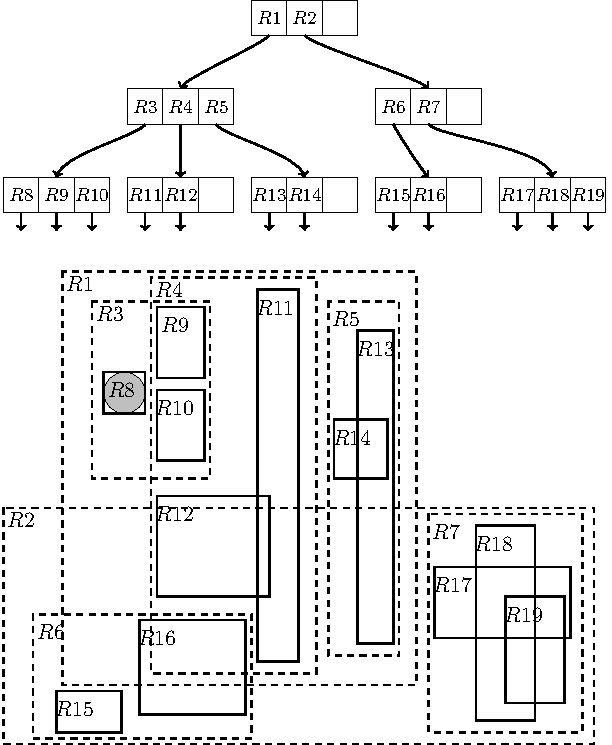
\includegraphics[scale=0.8]{figures/rtree.pdf}\\
\caption{R树示意图}{R tree illustration}
\label{fig:rtree}
\end{figure}

(1)R树插入

作为B树的一个变种,R树的插入与B树相类似,首先根据待插入空间对象的最小外包矩形待确定插入的叶节点,
然后插入对象,如果该叶节点包含的空间对象数目超过规定的最大数目,则将该节点进行分裂\cite{Huang2001Optimizing},并
将其中的一个节点向上传递,递归执行,如果直至根节点,完成树高度的提升。节点分裂的好还的标准是两个新节点的最小外包
矩形的面积之和最小。

(2)R树查询

R树查询只能检索出与给定窗口相交的空间实体对象。如果两个最小外包矩形是分离的,那么他们所代表的空间实体也肯定
是分离的,但如果两个最小矩形有相交,不能保证所包含的空间几何实体能够窗口相交。因此,R树空间检索检索策
略是:

过滤:从R树中筛选出候选节点,排除那些的不能满足相交条件的几何对象,但在候选几何对象中也
可能包含一些不满足条件的对象。由于判断最小外包矩形是否相交的计算成本低,可大幅度提高计算效率。

精选:依次判断每个候选几何对象,判断与查询窗口是否相交。可以借助JTS Topology Suite工具判断几何对象之间的拓扑关系。

在Spatial-Spark框架中,为了加快空间分析的速度,可选择在RDD的每个分区建立R树空间索引。通过RDD的MapPartition函数
将同一分区的空间对象汇集起来,每个分区建立一棵R树,将同一分区的几何对象的最小外包矩形插入树中。
通过Spark缓存机制,将索引内容缓存到Spark内存中,方便后续查询分析等工作。

\subsection{空间数据查询}

空间查询是GIS中最重要组成部分,在大规模空间数据中查询也提出了空间数据查询实时性要求。Spatial-Spark
在Spatial-RDD上层提供了空间查询层,包括空间拓扑查询(Spatial Topology Query),空间k邻居
查询(Spatial k Nearest Neighbor Query)和空间链接查询(Spatial Join Query)。使用者向
查询层发起空间查询请求,Spatial-Spark将查询的结果返回。如果空间数据在Spatial-RDD层事先建
立的了索引,那么用户可以借助索引,提高查询速度。

\subsubsection{空间拓扑查询}
空间拓扑关系是空间分析的特色,空间拓扑查询过程是给定一个空间几何对象和空间拓扑关系条件,从特定的
空间数据集筛选出符合条件的空间数据。

平面空间实体对象引入空间实体外部、内部和边界,构成了空间实体的基本组件。假设空间实体$A$的边界$\partial A$,
内部为$A^{\circ}$,补为$A^{-}$,空间实体$B$的边界为$\partial B$,内部为$B^{\circ}$,补为$B^{-}$,两两的交集就构
成了空间关系描述的9元组矩阵\cite{谢俊平2012拓扑关系和方向关系的统一表达模型}。
\[ R(A,B) = 
\begin{bmatrix}
\partial A \cap \partial B & \partial A \cap B^{\circ} & \partial A \cap B^{-} \\
A^{\circ} \cap \partial B & A^{\circ} \cap B^{\circ} & A^{\circ} \cap B^{-} \\
A^{-} \cap \partial B & A^{-} \cap B^{\circ} & A^{-} \cap B^{-} \\
\end{bmatrix}
\]

矩阵中每一个元素的取值都有空集和非空集两种,9个元素共存在512中可能,当然其中绝大部分
的空间拓扑关系时不存在的。以点、线和面为准给出所有可能空间对象之间可能拓扑关系,见表\ref{tab:geometrytopo}。
\begin{table}
  \centering
  \caption{空间几何拓扑关系}{Geometry topology rules}
  \label{tab:geometrytopo}
  \tabulinesep=1.5mm
  \begin{tabu}to 0.7\linewidth{X[1, c]X[1.2,c]X[1.2,c]X[1.2,c]}
    \tabucline[0.10em]-
    几何对象 & 点 & 线 & 面 \\
    \tabucline-
    点 & Equal\par Disjoint & Within\par Disjoint & Within\par Touch\par Disjoint \\
    \tabucline-
    线 & Contain\par Disjoint & Equals\par Within\par Overlap\par Contain\par Disjoint\par Intersect\par 
      & Within\par Disjoint\par Touch\par Intersect \\
    \tabucline-
    面 & Contain\par Disjoint & Contain\par Disjoint\par Touch\par Intersect\par &
    Equal\par Within\par Disjoint\par Touch\par Intersect\par Overlap\par Contain\par \\
    \tabucline[0.10em]-
  \end{tabu}
\end{table}

RDD中的filter算子可以筛选RDD中符合条件的元素,Spatial-Spark实现了Function接口的
通用空间拓扑查询类。该类接受待查询的空间元素Geometry和待判断的空间拓扑关系条件Condition。在
类中重写call函数即可,通用实现如下。
\begin{lstlisting}[language=Java]
@Override
public Boolean call(Geometry goe){
    return geo.condition(this.query)
}
\end{lstlisting}


当在Spatial-RDD中如果已经在每个分区构建好R树索引,可以通过索引查询相交(Intersect)、包
含(Contain)、相等(Equal)、重叠(Overlap)和被包含(Within)的拓扑关系。RDD中的FlatMapPartition算子
可以对每个分区进行操作,并将结果展平(Flat)返回,用户定义Spatial-Spark预先实现了FlatMapFunction接
口的类,该类构造函数只包含带查询对象的最小外包矩形(Envelope),通过R树高效的查询函数返回最小外包矩形与待查询
的外包矩形的空间几何对象。索引查询是初步空间查询,在返回的结果中,在对数据进行精确空间拓扑查询,通用实现如下。
\begin{lstlisting}[language=Java]
@Override
public Iterator<Geometry> call(Iterator<STRTree> t){
    STRtree tree = t.next()
    return tree.query(this.query.getEnvelopeInternal())
}
\end{lstlisting}

\subsubsection{空间k邻居查询}
空间K个近邻居查询在现实生活中有着广泛应用,尤其在移动互联网时代,位置推荐、商场选址和公共交通等方面有着
广泛应用\cite{董亭亭2013大数据下空间数据索引和}。Spatial-Spark在K邻居查询,算法借助优先级队列数据结构,
算法主要分为两步:\circled{1}选择:针对每个分区,接受一个查询点和查询邻居数量K,在该分区中,构建一个容量
为K的优先级队列,依次将计算查询点与分区内几何对象的空间欧氏距离,并添加至优先级队列中,如果队列已满,将
集合中距离最大元素删除再添加;\circled{2}合并:针对每个分区的优先级队列,再次筛选出前K个最小距离的几何
要素,KNN通用查询类如下。
\begin{lstlisting}[language=Java]
@Override
public Iterator<Geometry> call(Iterator<Geometry> inputs){
        while(inputs.hasNext()){
            if(pq.size()< this.k){
                pq.offer(inputs.next());
            }else{
                Geometry geo = inputs.next();
                double distance = geo.distance(this.query);
                double longestDistance = pq.peek().
                                    distance(this.query);
                if(longestDistance > distance){
                    pq.poll();pq.offer(geo);
                }
            }
        }
}
\end{lstlisting}


\subsubsection{空间连接查询}
空间连接查询是常用且复杂的空间数据查询操作,类似于数据库的两张表Join查询,从两个空间对象集合中查询出符合特定空间关
系的空间几何对象对\cite{Jacox2007Spatial}。例如两个空间数据集A和B,空间连接是从A中的空间对象到B中的空间对象使用空间拓扑
关系$t$,返回分别来自A和B的满足条件的几何对象对,空间对象的复杂性和海量性将会导致空间连接运算需要大量的
计算,时间复杂急剧上升。Spark的并行计算特点为空间连接运算提供了新的模式,因此Spatial-Spark采用了并
行化方式实现了空间连接查询算法。算法的主要步骤分为两步。

(1)过滤步骤

借鉴Spatial-Spark空间分区算法,首先将其中任意空间数据集的边界按其最小的几何对象外包
矩形分割成规则的网格,每个网格赋予编号。将空间数据集的每一个元素与判断与之相交的最小外包矩形
编号,通过RDD相应的MapToPair操作转换成PairRDD,其中键key为网格的编号,值value为空间几何对象,再使
用转换函数cogroup,按照key将连个要素集合并起来。
\begin{figure}
\centering
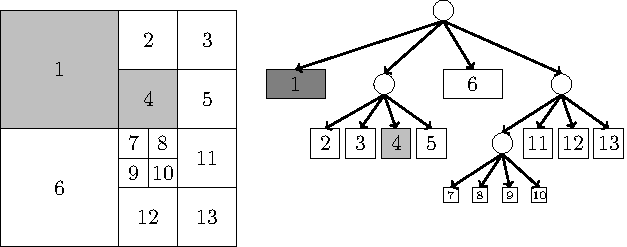
\includegraphics[scale=0.8]{figures/quadtree.pdf}
\caption{四叉树示意图}{Quadtree illustration}
\label{fig:quadtree}
\end{figure}


在空间元素最小外包矩形与格网相交时,可以预先将整个格网数据进行预处理。四叉树也是一种树状索引数据
结构,地理空间对象局部范围信息可以用四叉树进行存储,其采取从整体到局部划分的方式建立索引。建立过程
如下:对空间范围平面平均分成四个部分,如果改部分的空间对象属性一致,则不再划分,否则继续划分四个小
部分,如此重复递归执行。每划分一次,四叉树深度增加1,对于深度为$n$的四叉树索引,包含的空间对象至多为($2^n \times 2^n$)个,
四叉树示意图见\ref{fig:quadtree}。

对于空间连接查询中预先处理的格网建立的四叉树索引,所有的叶节点的深度相同,平均每次查询的时间复杂
度为$\log_{4}n$,而遍历整个格网的时间复杂度为$n$。

(2)求精步骤

在过滤阶段中,同一网格内空间对象,再根据空间拓扑要求精确筛选,返回结果中每个元素表示
一对满足条件的空间拓扑要求的几何对象对,整个空间连接过程见算法\ref{alg:join}。
\begin{algorithm}[h]   
\caption{空间连接查询}
\label{alg:join}
\begin{algorithmic}[1] %这个1 表示每一行都显示数字  
\REQUIRE  ~~\\ %算法的输入参数:Input  
空间RDD1:spatial\_rdd1;\\  
空间RDD2:spatial\_rdd2;\\  
\ENSURE ~~\\ %算法的输出:Output  
空间连接对象对, spatial\_join; \\
\STATE $//$与网格相交生成key-value;
\STATE spatial\_pair\_rdd1 = spatial\_rdd1.flatToPair(); \\ 
       spatial\_pair\_rdd2 = spatial\_rdd2.flatToPair();
\STATE $//$按key进行cogroup操作;

\STATE spatial\_pair\_groups = spatial\_pair\_rdd1.cogroup(spatial\_pair\_rdd2);

\STATE $//$每个value进行详细拓扑判断

\STATE spatial\_pair\_values = spatial\_pair\_groups.mapValue();  

\STATE $//$去重操作 
\STATE spatial\_pair\_join = spatial\_pair\_values.reduceByKey(); 
\STATE $//$去掉key 
\STATE spatial\_join = spatial\_pair\_join.mapToPair(); 
\RETURN spatial\_join; %算法的返回值  
\end{algorithmic}  
\end{algorithm} 


\section{Spatial-Spark实验分析}{Experiments and Analysises of Spatial-Spark}

\subsection{实验平台及配置}
为了验证Spatial-Spark计算框架在空间数据分析中的优势,搭建了Hadoop/Spark计
算集群\cite{Ghosh2017Install1, Ghosh2017Install2},整个集群有$10$台服务器组成,
每台服务器安装了VMware虚拟机,每台虚拟机使用的操作系统为Centos $6.4$ Linux操作
系统,每台虚拟机的配置见表\ref{tab:clusterconfig}:
\begin{table}
  \centering
  \caption{集群配置}{Cluster configurations}
  \label{tab:clusterconfig}
  \tabulinesep=1.5mm
  \begin{tabu}to 0.5\linewidth{X[1, c]X[1,c]}
    \tabucline[0.10em]-
    项目 & 配置  \\
    \tabucline-
    内存 & $4$G \\
    CPU核心 & 双核四线程 \\
    硬盘容量 & $30$G \\
    操作系统 & CentOS $64$位 \\
    Hadoop版本 & $2.6$ \\
    Spark版本 & $1.4$ \\
    JDK & $1.7$ \\
    以太网络 & $1000$Mbps \\
    \tabucline[0.10em]-
  \end{tabu}
\end{table}

Hadoop/Spark集群部署繁琐,涉及到各个方面的技术,其中包括Linux系统的配置,Hadoop的配置与
调试,Java和Scala语言库的安装,Spark计算框架配置和部署。 为了能够使集群能够相互通信,对
$10$台服务器IP地址划分和Hostname修改,因为集群之间需要进行数据交换处理,所以要配置使节点之
间能够SSH免密码通信。各节点IP配置见表\ref{tab:ipclusterconfig}:
\begin{table}
  \centering
  \caption{节点IP}{Nodes' IP addresses}
  \label{tab:ipclusterconfig}
  \tabulinesep=1.5mm
  \begin{tabu}to 0.8\linewidth{X[1,c]X[1,c]|X[1, c]X[1,c]}
    \tabucline[0.10em]-
    节点 & IP地址 & 节点 & IP地址  \\
    \tabucline-
    Master & $192.168.5.100$ & Node$5$ & $192.168.5.105$ \\
    Node$1$ & $192.168.5.101$ & Node$6$ & $192.168.5.106$ \\
    Node$2$ & $192.168.5.102$ & Node$7$ & $192.168.5.107$ \\
    Node$3$ & $192.168.5.103$ & Node$8$ & $192.168.5.108$ \\
    Node$4$ & $192.168.5.104$ & Node$9$ & $192.168.5.109$ \\
    \tabucline[0.10em]-
  \end{tabu}
\end{table}

其中Master节点为主节点,守护Hadoop的Namenode进程、Yarn的ResourceManager进程和Spark的
Master进程。而Node$1\sim $Node$9$节点为从节点,守护Hadoop的Datanode进程和Spark的Worker进程,其
中Node1节点另外守护Hadoop SecondaryNameNode进程,当Master节点的Namenode进程出现
故障,Node$1$节点将被担当起NameNode节点的作用。

Spark计算模式主要分为三种:Local模式、Standalone模式和Yarn-Cluster模式。Local模式是在
本地运行,Spark的Local模式部署简单,适合单机上调试编写的Spark 应用程序;Standalone模式
是Spark自身实现资源调度框架\cite{Fern2016Automated},当不需要其他计算框架的时候如MapReduce、Storm等,只使用
Spark进行大数据计算时,可以采用Standalone模式,其中Spark Shell交互式运行环境就是运行在
该模式之上;Yarn-Cluster模式借助Yarn统一管理整个计算资源,用户在Yarn集群中的服务和Spark
应用的资源完全隔离。

为了方便调试,本实验采用Standalone模式,当整个集群配置完毕后,启动Spark-Shell,采用Scala
交互式语言编写WordCount程序,返回正确结果表明整个hadoop-spark集群配置成功。
\subsection{实验对比分析}

(1)MapReduce与Spatial-Spark空间过滤筛选对比

在相同的集群中,分别编写MapReduce应用程序和Spatial-Spark应用程序,对相同规模的空间数据进
行空间数据分析。选用的数据为全国所有道路线状空间对象(包括高速公路、国道、省道、县道),首先
对原有的ShapeFile数据转换成OGC标准的WKT文件,按行存储为一个空间对象,在集群中通过Hadoop相关命
令,存放到HDFS中,集群中HDFS的Block的大小为$128$M。空间过滤算法定义为选择其中一条道路,求解
其外包矩形中包含的所有其他道路。

实验分为五组,实验数据量分别为$200$M、$500$M、$1$G、$2$G和$3$G,结果见图\ref{fig:topycomparsion},当数据量不大的
时候,Spatial-Spark相对于MapReduce优势不够明显,当数据量达到一定程度后,Spatial-Spark内存
计算的优势突显出来,在相同的条件下,MapReduce消耗的时间是Spatial-Spark的两个数量级。
\begin{figure}
  \centering
  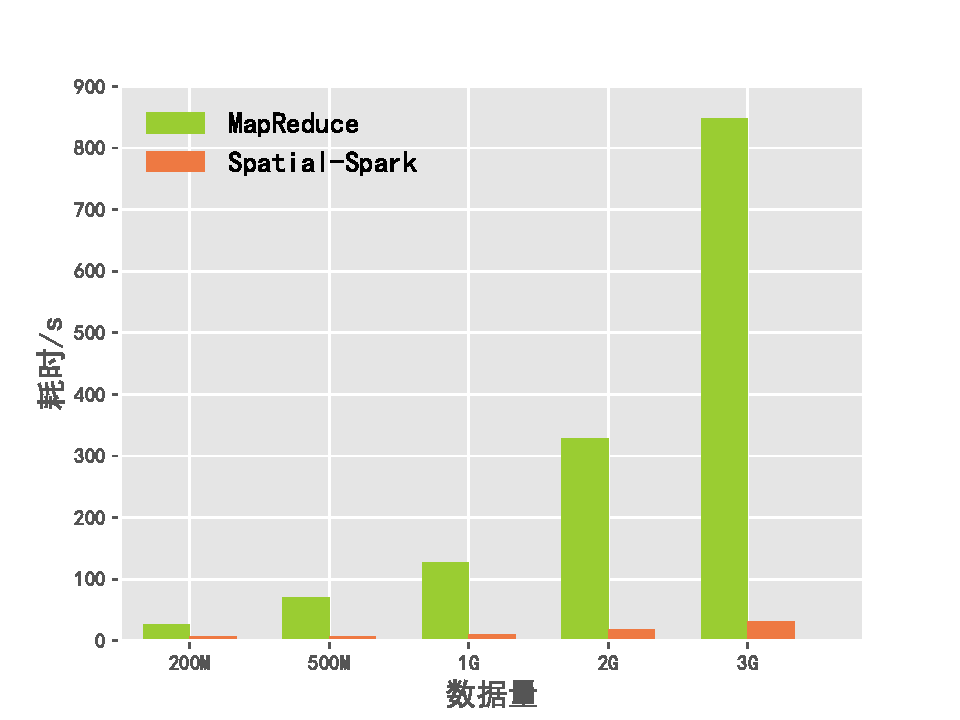
\includegraphics[scale=0.7]{figures/topo_query.pdf} \\
  \caption{MapReduce和Spatial-Spark查询对比}{MapReduce and Spatial-Spark topology query comparsion}
  \label{fig:topycomparsion}
\end{figure}

(2)Spatial-Spark集群扩展性能分析

Spatial-Spark计算框架的优越性在于其横向扩展性(Scale Out),通过增加廉价的计算机,使得
计算性能呈现显著性增加。在空间大数据分析中也不例外,本实验通过分析动态调整工作节点的
数目,比较在相同的数据规模下各个不同工作节点数目下,消耗的时间对比。

空间连接查询是空间运算中计算量较大的运算,选用的数据为全国县界面对象,共2917个面对象,与
全国道路中进行连接操作,获取每个县与之相交的道路。

实验共分为四组,使用的Work Node的数量分别为$2$、$4$、$6$和$8$,实验数据量$150$M县界对象,$1$G的全国道
路。为实验结果见图\ref{fig:node_memory},第一组实验引发java.lang.OutOfMemoryError异常,集群内存不足。其余
实验组时间消耗大致相同。

内存大小也是影响Spatial-Spark运算速度中重要因素,Spark在提交任务时候,可以通过executor-memory参数指
定每个工作节点提供给本次计算的内存,Standalone工作模式将会统一管理这些内存和资源调配。通过调整
内存参数,分析空间链接操作耗时。
\begin{figure}
  \centering
  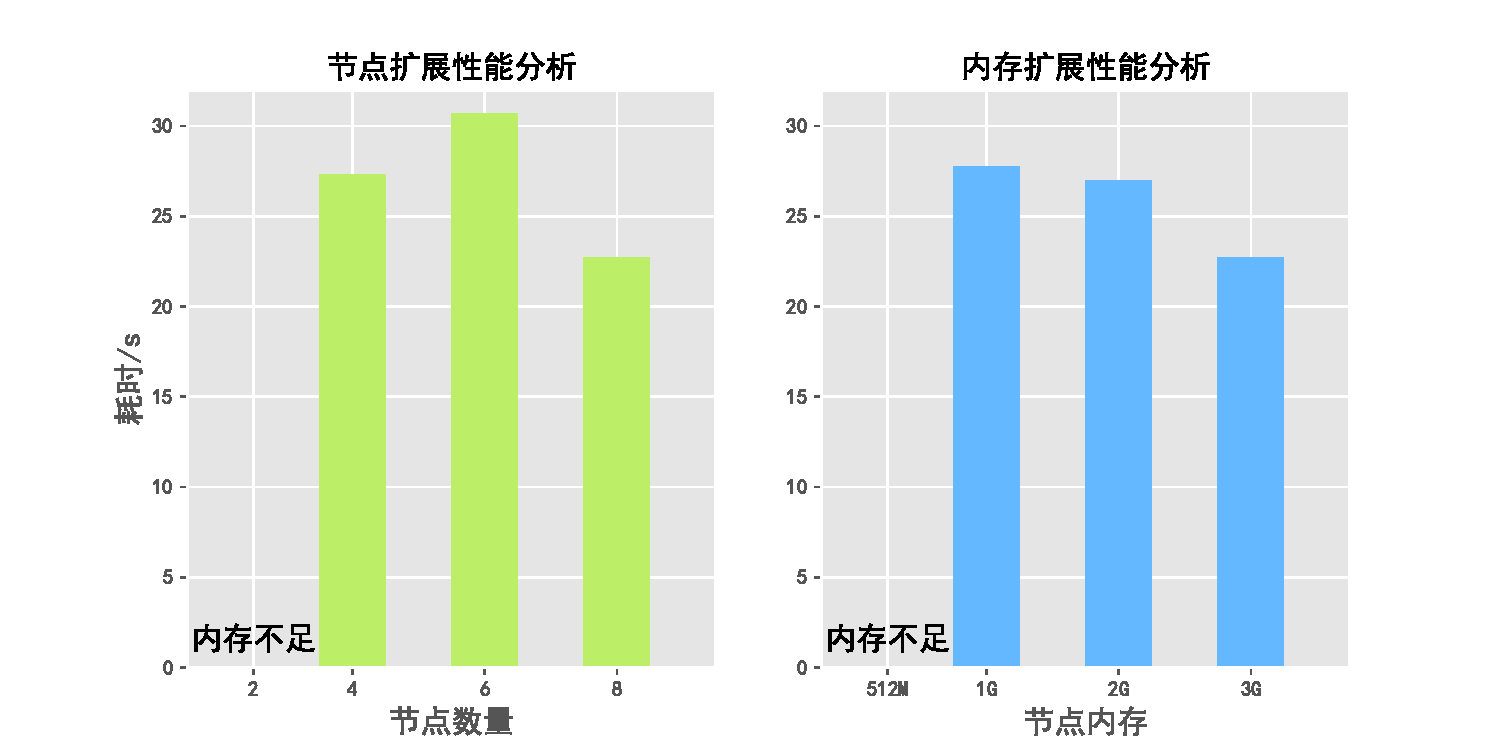
\includegraphics[scale=0.5]{figures/node_memory.pdf} \ \
  \caption{Spatial-Spark扩展性实验}{Spatial-Spark scale-out results}
  \label{fig:node_memory}
\end{figure}

实验共四组,每一组节点的内存分别为$512$M、$1$G、$2$G和$3$G,实验数据量$150$M县界对象,$1$G的全国道路。实验结
果见图\ref{fig:node_memory},第一组实验引发java.lang.OutOfMemoryError异常,集群内存不足。其余实验随着集群内存
的增大,时间消耗也呈下降趋势。

(3)Spatial-Spark空间索引性能分析

Spatial-Spark不仅仅是RDD的空间拓展,而且在分布式空间计算中引入了空间索引,并将索引通过Spark存
储策略缓存在内存中,并根据空间数据的分区,为每个分区建立了索引。由于R树索引存储的为空间对象的最
小外包矩形,因此在相关空间分析时,需要在初步筛选后进行精确空间判断分析。
\begin{figure}
  \centering
  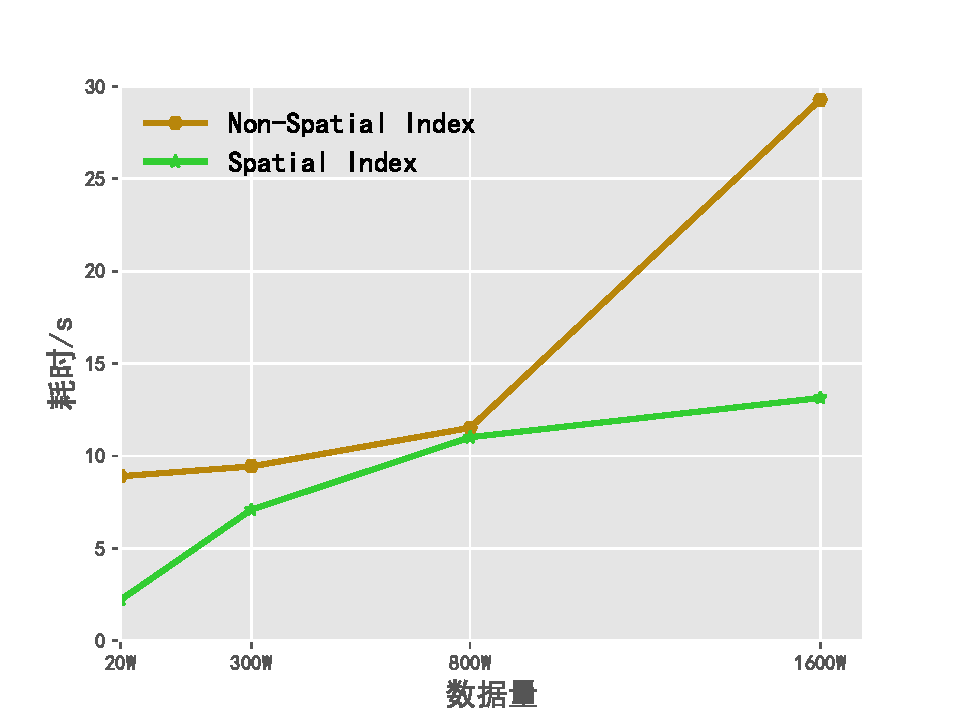
\includegraphics[scale=0.7]{figures/index.pdf} \\
  \caption{Spatial-Spark索引和非索引比较}{Spatial-Spark index Vs. non-index query comparsion}
  \label{fig:index}
\end{figure}

KNN空间查询是常用的空间数据查询分析,选择全国兴趣点(POI)共八百多万条数据,共$2.3$G,按行存储
数据,包含了空间和非空间数据。

实验总共分为四组,POI数目分别为$20$W、$300$W、$800$W和$1600$W,结果见图\ref{fig:index},对已经建立空间索引的KNN
查询消耗时间比非空间索引少,随着数据量增加,空间索引优势越发明显。
\subsection{Spatial-Spark优化方案}

Spark程序都具有「内存计算」的天性,所以集群中的所有资源:CPU、网络带宽或者内存都是成为Spark程序性能的瓶颈。

(1)数据序列化

序列化的作用是能够将数据在集群网络传输,因此序列化的对于提高分布式程序的性能起到重要的作用,一个不
好的序列化方式将会极大地降低计算速度。因此优化对象的为提高Spark应用程序的第一选择\cite{Zhao2016An}。Spark提供
了两种序列类库: \circled{1} Java序列化:在默认情况下,Spark采用Java的ObjectOutputStream序列化一个对象,只要
类实现了java.io.Serializable接口。Java序列化十分灵活方便,但是速度较慢;\circled{2}Kryo序列化:Spark也
能使用Kryo序列化对象,Kryo不仅速度快,而且生成的结果更为紧凑。但Kryo序列化使用比较繁琐,需要提
前注册要序列化的类。

在Spatial-Spark中,实验表明使用Java序列化对象某一RDD消耗为$434$M内存,当改用Kryo序列化后占该
RDD消耗$53$M内存,优化效果明显。

(2)内存优化

Spark内存计算给大数据分析带来了便利,但针对特别大的分析数据,内存无法完整加载,RDD持久化API提
供了多种序列化存储级别,见表\ref{tab:level},不同的序列化选择,使得在处理大数据时在效率和内存之间选择不同的权衡。

\begin{table}
  \centering
  \caption{存储级别策略}{Storage level stragies}
  \label{tab:level}
  \tabulinesep=1.5mm
  \begin{tabu}to 0.8\linewidth{X[1, c]X[1,c]}
    \tabucline[0.10em]-
    存储级别 & 说明  \\
    \tabucline-
    MEMORY\_ONLY & 全部序列化到内存 \\
    DISK\_ONLY & 全部序列化到磁盘 \\
    MEMORY\_AND\_DISK & 序列化到内存和磁盘 \\
    MEMORY\_ONLY\_SER & 序列化到内存字节数组 \\
    \tabucline[0.10em]-
  \end{tabu}
\end{table}

用多大内存来缓存数据是内存回收是非常重要的参数,在默认情况下,Spark采用运行内存
的$60\%$空间来进行RDD缓存,所以在程序运行期间只有$40\%$的内存可以用来创建对象。当程序运行过程中JVM频
繁进行垃圾回收,会大大减低程序运行速度,为了提高效率,可以手动修改缓存大小比例。

\section{本章小结}{Chapter Summary}

本章着重介绍了Spatial-Spark大数据空间分析框架,首先分析了矢量空间数据格式种类,空间数据转换和开源空间
数据分析包;接着对Spark核心数据结构RDD空间扩展为Spatial-RDD,并着重对空间数据进行空间分区索引,
以此为基础,构建了常见空间分析应用API。以实验为基准,分析了Spatial-Spark的性能方面的特点。
